\chapter{Análisis de duracion de tiempos constantes de los estados}\label{A:T_cte}

Para poder realizar una comparación justa con el modelo con ley de potencia en el tiempo que pasa en ambos estados, es necesario mostrar las métricas a medida que se agregan 
los mismos condimentos que en el modelo troncal de la tesis. Las capas se agregan en el siguiente orden: Primero el ruido del GPS, luego se utiliza la variación en la hora 
en la que comienza a caminar, para finalmente agregar una variación en la velocidad constante del día.

\section*{$1^{\text{era}}$ Configuración: tiempo de caminata constante}


A continuación, en la Figura~\ref{fig:Cte_W}, mostramos como evolucionan las métricas a medida que se agregan las distintas partes del modelo. Para cada una de 
las modificaciones se ajustó la velocidad y la variación angular que mejor ajuste el MSD y el P(d)

\begin{figure}[H]
    \centering
    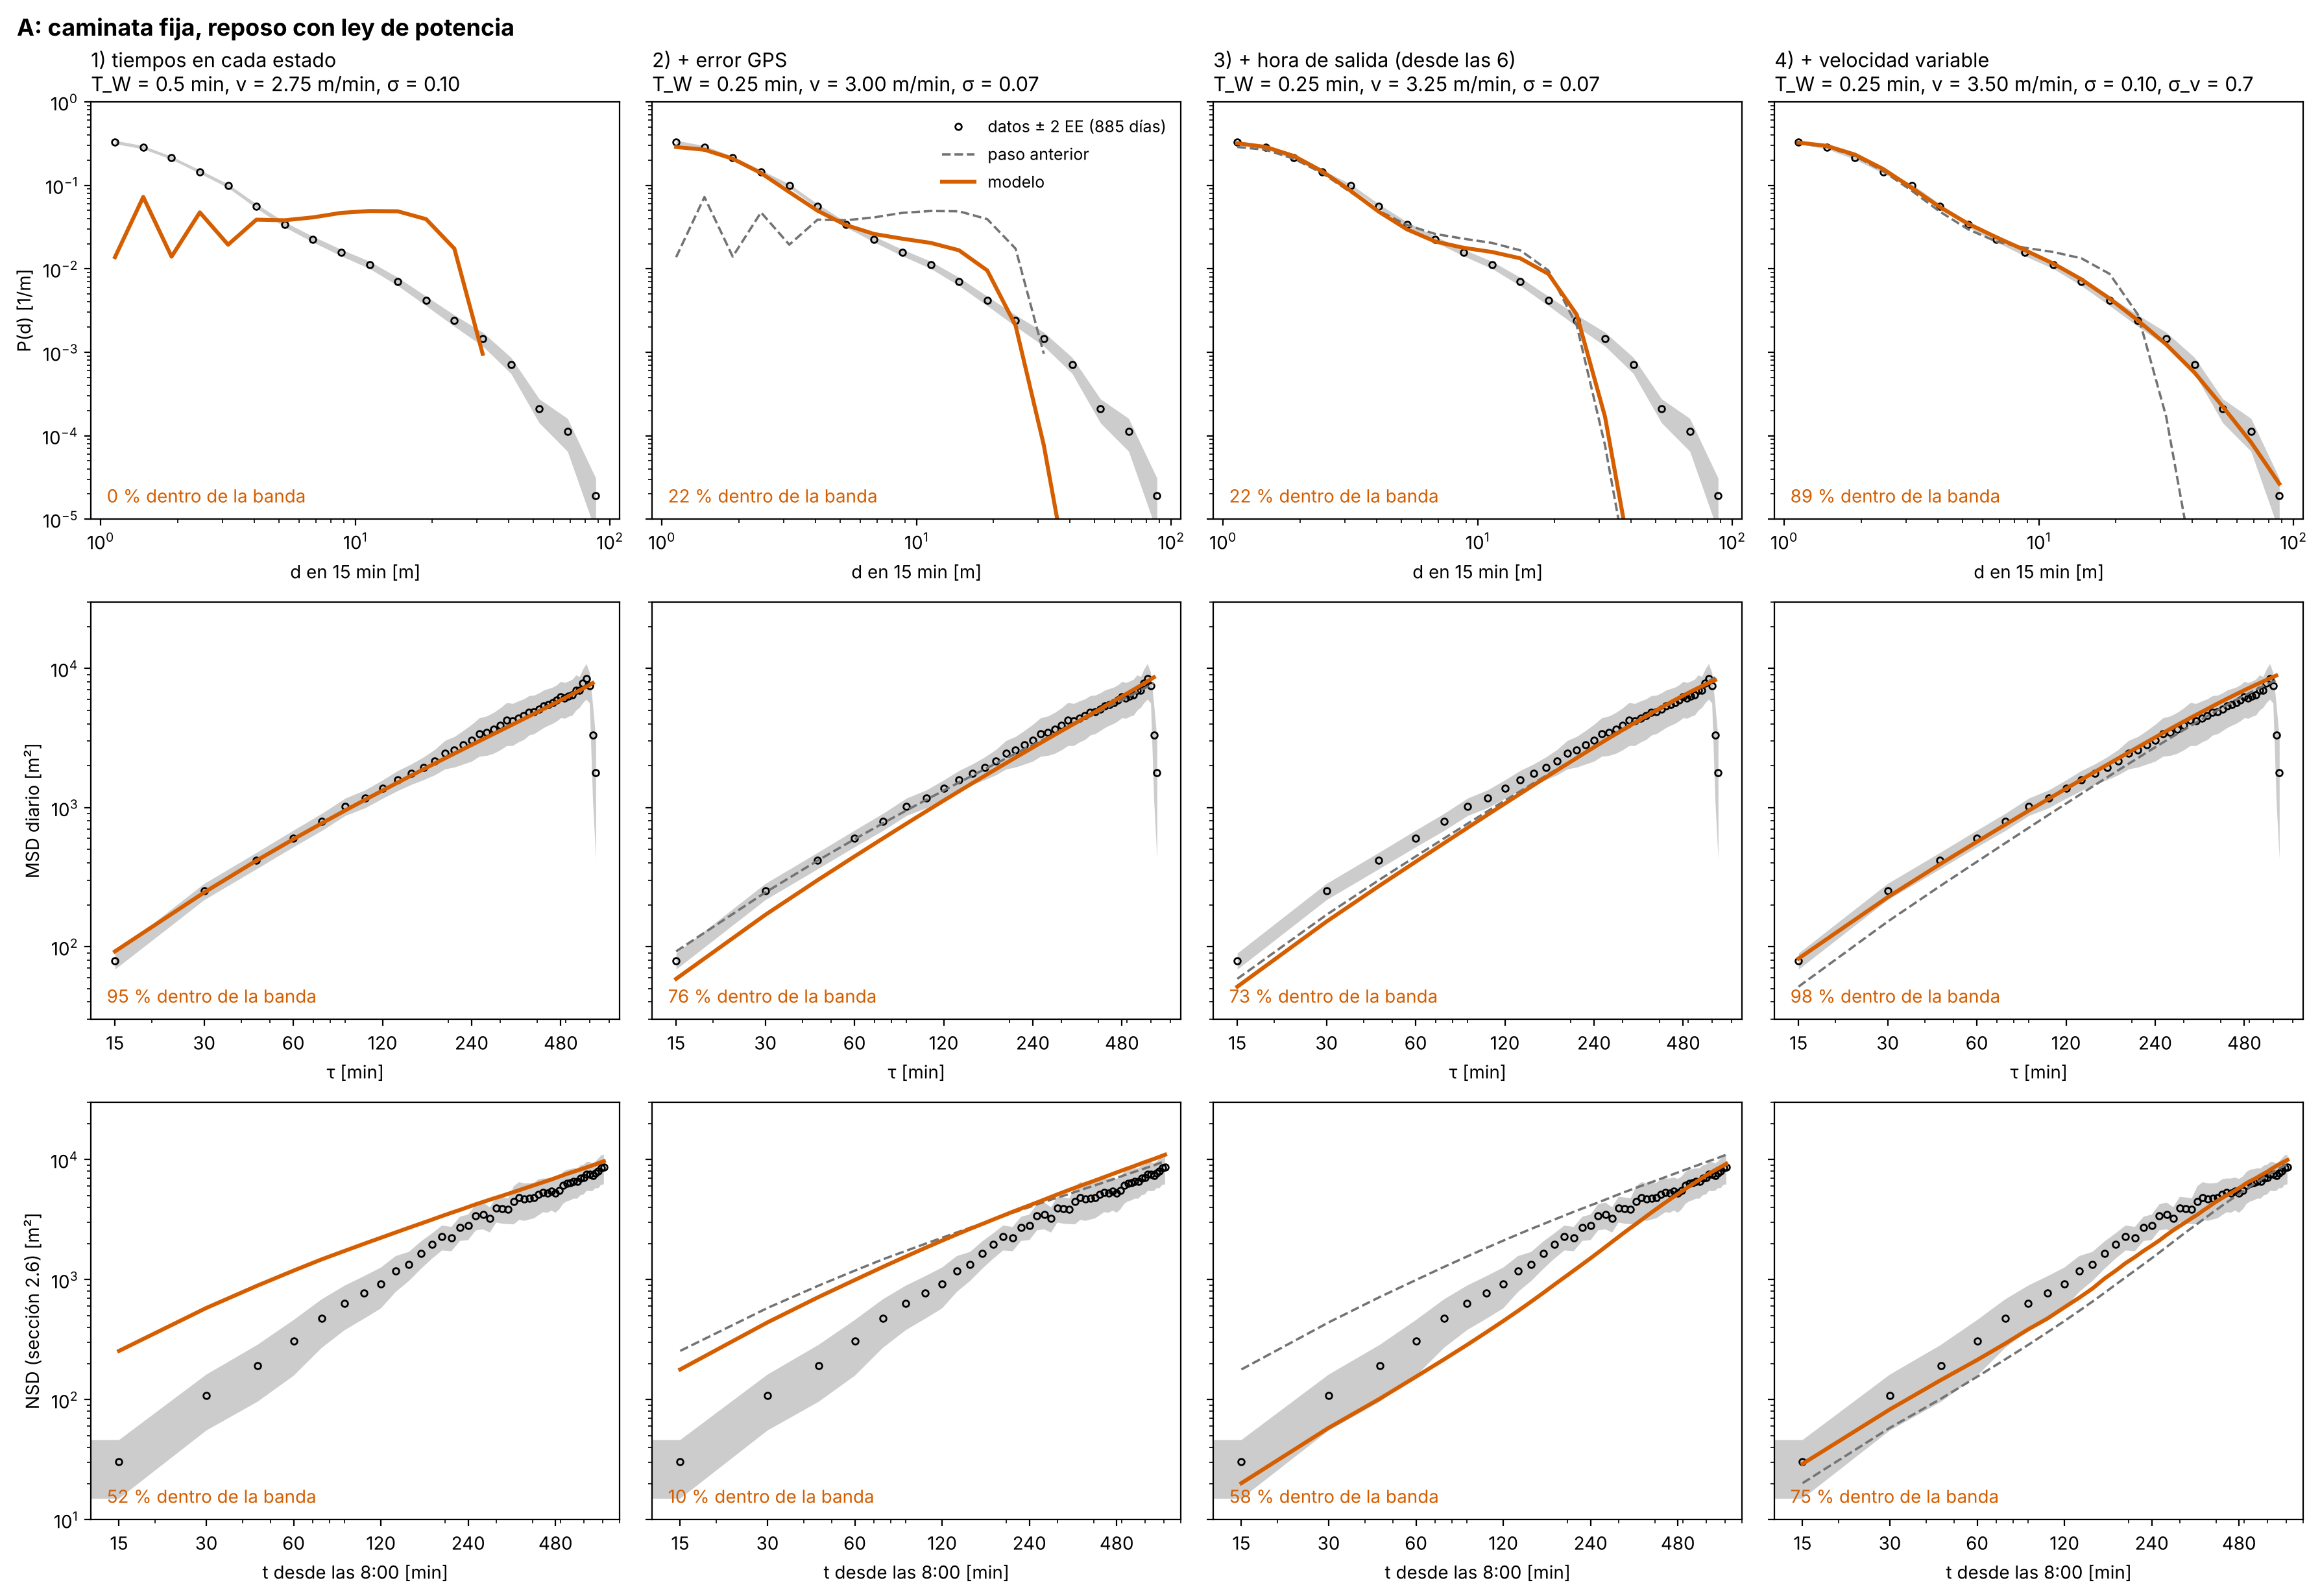
\includegraphics[width=0.95\textwidth]{CteW.png}
    \caption{Gráfico de evolución de las métricas a medida que se incorporan las distintas capas del modelo con tiempos de caminata constantes.}
    \label{fig:Cte_W}
\end{figure}

Podemos observar que el modelo tiene la capacidad de replicar en buena medida las métricas obtenidas de los datos

\section*{$2^{\text{da}}$ Configuración: tiempo de reposo constante}

Para esta segunda configuración, fijamos el tiempo de reposo constante y dejamos que el tiempo de caminata siga una ley de potencia. En la Figura~\ref{fig:Cte_S},
repetimos el análisis que realizamos con tiempos de caminata constantes.

\begin{figure}[H]
    \centering
    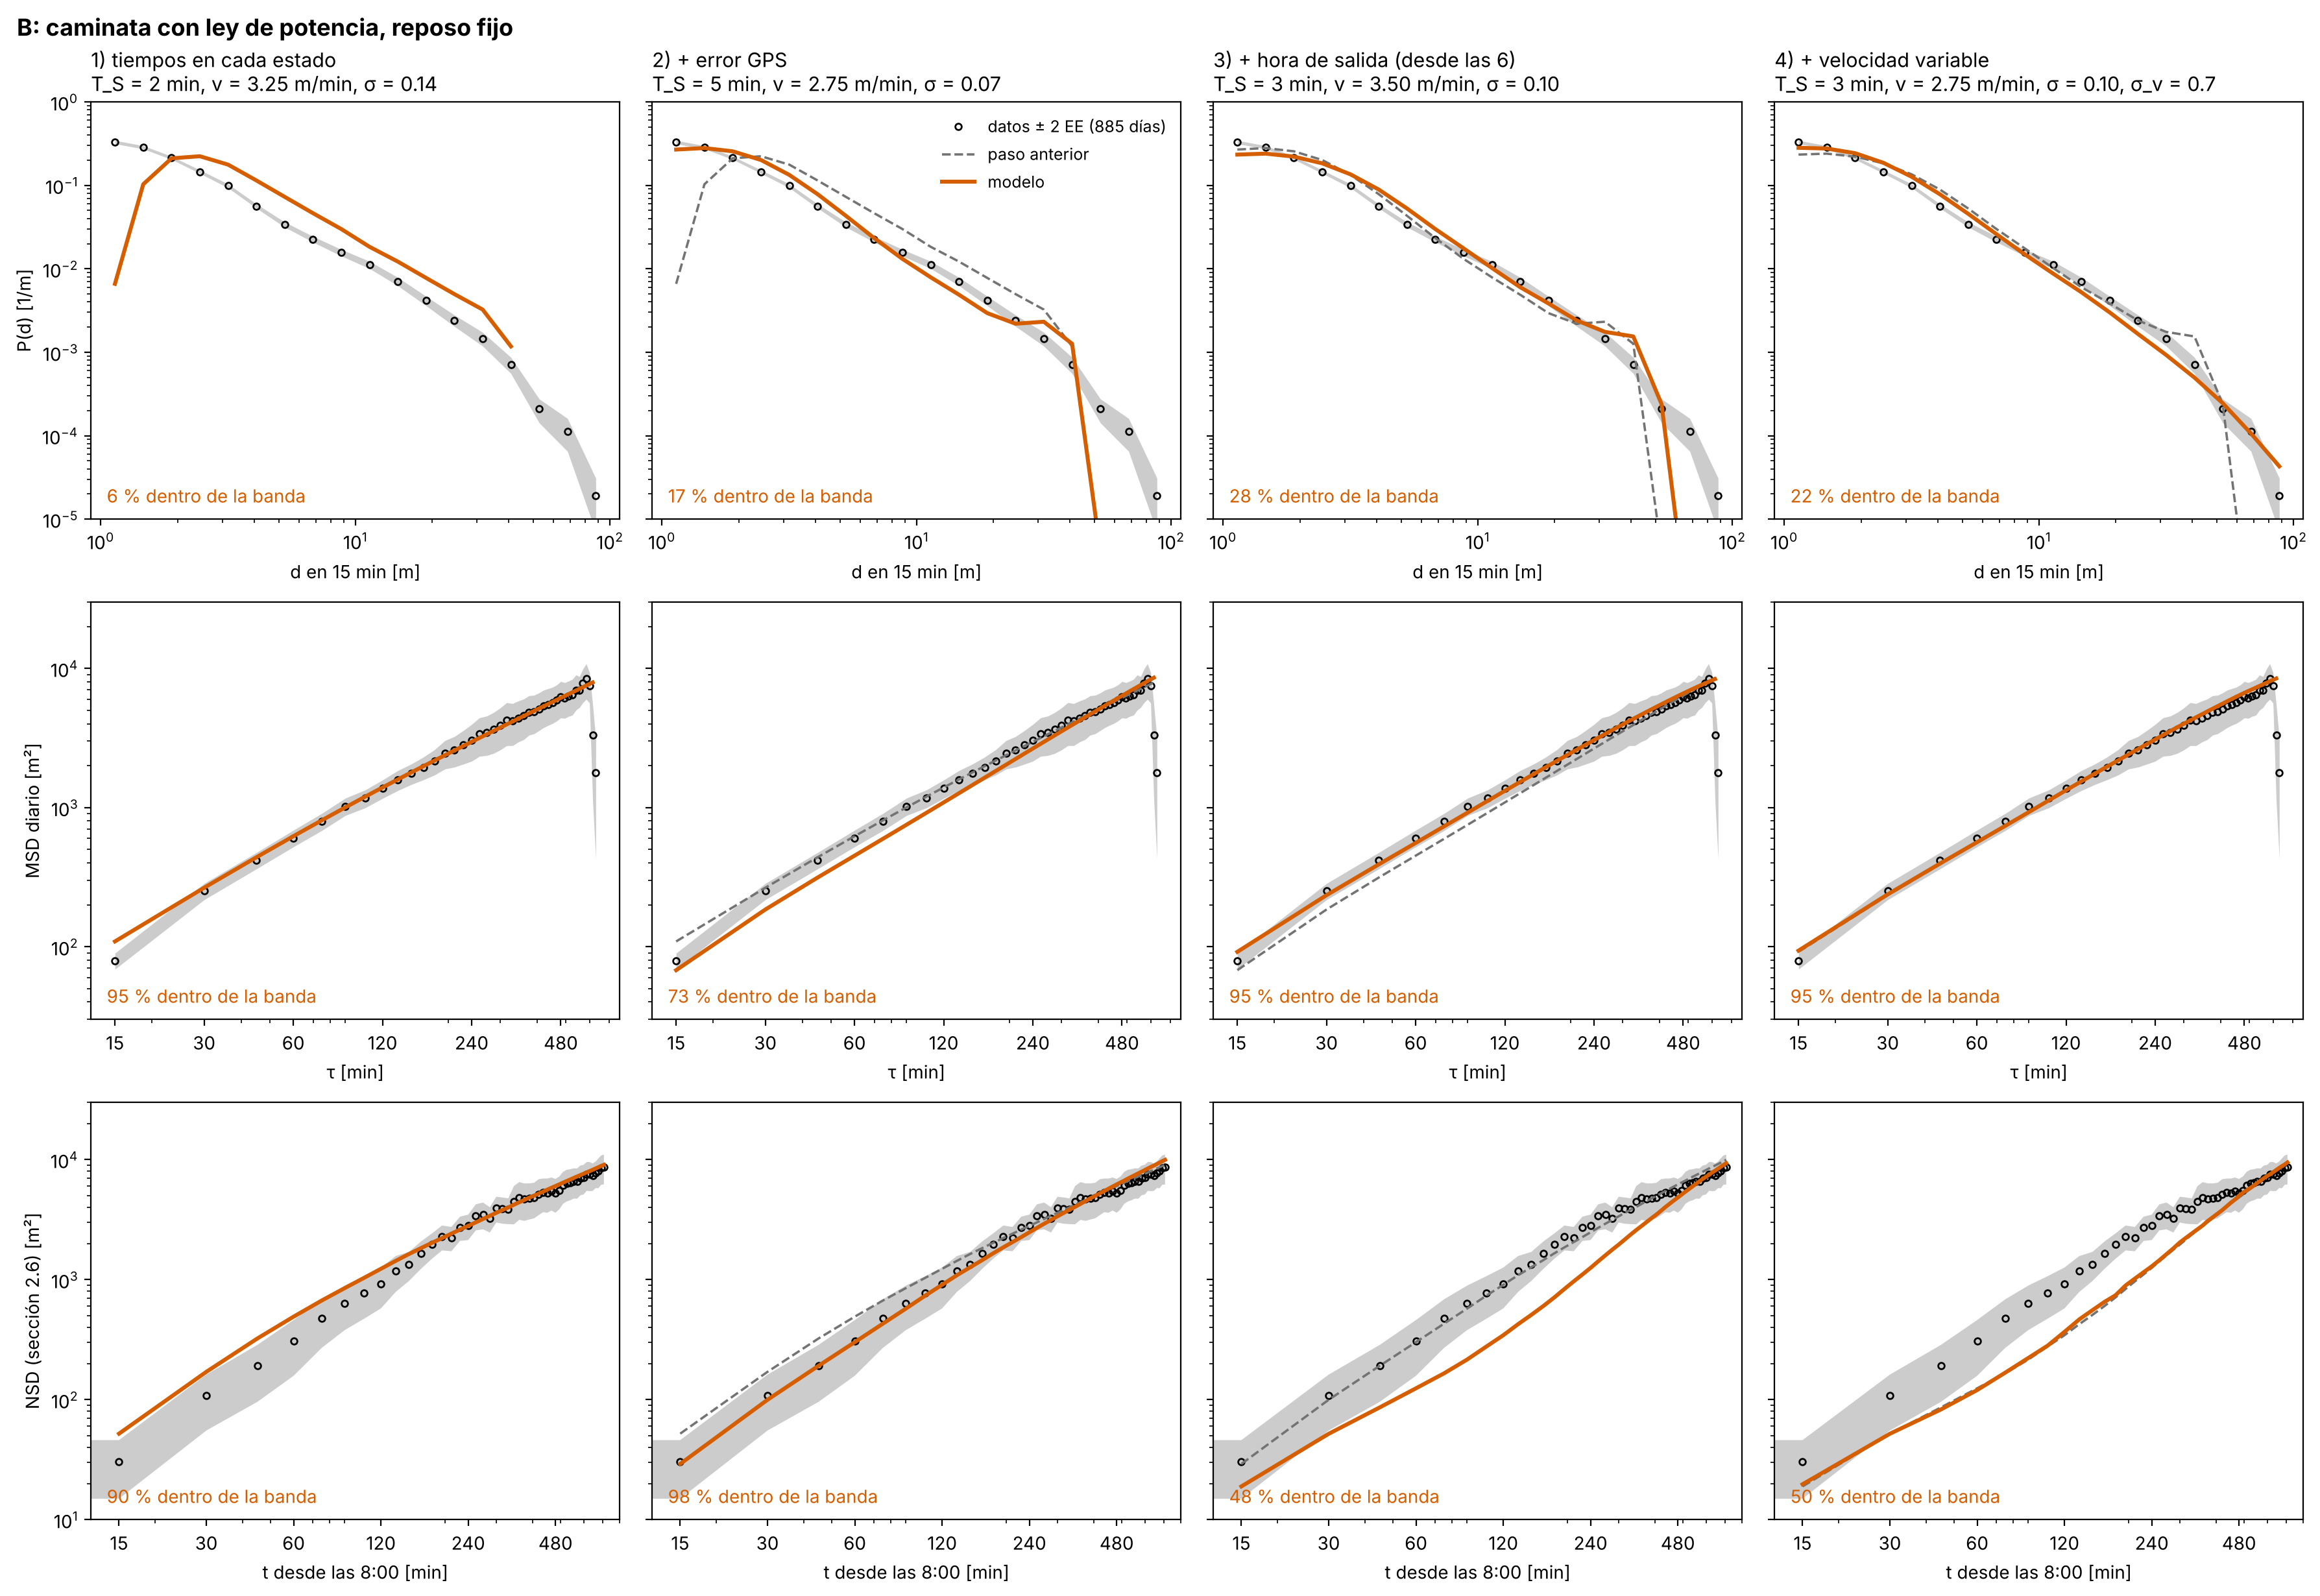
\includegraphics[width=0.95\textwidth]{CteS.png}
    \caption{Gráfico de evolución de las métricas a medida que se incorporan las distintas capas del modelo con tiempos de reposo constantes}
    \label{fig:Cte_S}
\end{figure}

Si bien el modelo parece fallar para la métrica del NSD, la cuál es muy ruidosa, conviene destacar la buena capacidad que tiene esta configuración para replicar
las métricas de P(d) y MSD diario.

\section*{Conclusión}

El descarte de estos modelos se debe principalmente a que al tener datos del acelerómetro se pudo medir en el trabajo de Callenbach~\cite{callenbach2025} 
que las distribucion de probabilidad de pasar cierto tiempo en estado de reposo o de caminata no sigue una delta hubicada en algún valor constante.
Si no fuera por esa información, no se haya suficiente información en los datos de GPS para elegir el modelo de leyes de potencia por sobre los presentados en este apéndice.

%%% Local Variables: 
%%% mode: latex
%%% TeX-master: "template"
%%% End: 
